%definira klasu dokumenta 
\documentclass[12pt]{report} 

%prostor izmedu naredbi \documentclass i \begin{document} se zove uvod. U njemu se nalaze naredbe koje se odnose na cijeli dokument

%osnovni LaTex ne može riješiti sve probleme, pa se koriste različiti paketi koji olakšavaju izradu željenog dokumenta
\usepackage[croatian]{babel} 
\usepackage{amssymb}
\usepackage{amsmath}
\usepackage{txfonts}
\usepackage{mathdots}
\usepackage{titlesec}
\usepackage{array}
\usepackage{lastpage}
\usepackage{etoolbox}
\usepackage{tabularray}
\usepackage{color, colortbl}
\usepackage{adjustbox}
\usepackage{geometry}
\usepackage[classicReIm]{kpfonts}
\usepackage{hyperref}
\usepackage{fancyhdr}

\usepackage{float}
\usepackage{setspace}
\restylefloat{table}


\patchcmd{\chapter}{\thispagestyle{plain}}{\thispagestyle{fancy}}{}{} %redefiniranje stila stranice u paketu fancyhdr

%oblik naslova poglavlja
\titleformat{\chapter}{\normalfont\huge\bfseries}{\thechapter.}{20pt}{\Huge}
\titlespacing{\chapter}{0pt}{0pt}{40pt}


\linespread{1.3} %razmak između redaka

\geometry{a4paper, left=1in, top=1in,}  %oblik stranice

\hypersetup{ colorlinks, citecolor=black, filecolor=black, linkcolor=black,	urlcolor=black }   %izgled poveznice


%prored smanjen između redaka u nabrajanjima i popisima
\newenvironment{packed_enum}{
	\begin{enumerate}
		\setlength{\itemsep}{0pt}
		\setlength{\parskip}{0pt}
		\setlength{\parsep}{0pt}
	}{\end{enumerate}}

\newenvironment{packed_item}{
	\begin{itemize}
		\setlength{\itemsep}{0pt}
		\setlength{\parskip}{0pt}
		\setlength{\parsep}{0pt}
	}{\end{itemize}}




%boja za privatni i udaljeni kljuc u tablicama
\definecolor{LightBlue}{rgb}{0.9,0.9,1}
\definecolor{LightGreen}{rgb}{0.9,1,0.9}

%Promjena teksta za dugačke tablice
\DefTblrTemplate{contfoot-text}{normal}{Nastavljeno na idućoj stranici}
\SetTblrTemplate{contfoot-text}{normal}
\DefTblrTemplate{conthead-text}{normal}{(Nastavljeno)}
\SetTblrTemplate{conthead-text}{normal}
\DefTblrTemplate{middlehead,lasthead}{normal}{Nastavljeno od prethodne stranice}
\SetTblrTemplate{middlehead,lasthead}{normal}

%podesavanje zaglavlja i podnožja

\pagestyle{fancy}
\lhead{Programsko inženjerstvo}
\rhead{Tectonic HR}
\lfoot{BitByBit}
\cfoot{stranica \thepage/\pageref{LastPage}}
\rfoot{\today}
\renewcommand{\headrulewidth}{0.2pt}
\renewcommand{\footrulewidth}{0.2pt}


\begin{document} 
	
	
	
	\begin{titlepage}
		\begin{center}
			\vspace*{\stretch{1.0}} %u kombinaciji s ostalim \vspace naredbama definira razmak između redaka teksta
			\LARGE Programsko inženjerstvo\\
			\large Ak. god. 2021./2022.\\
			
			\vspace*{\stretch{3.0}}
			
			\huge Tectonic HR\\
			\Large Dokumentacija, Rev. \textit{2}\\
			
			\vspace*{\stretch{12.0}}
			\normalsize
			Grupa: \textit{BitByBit}\\
			Voditelj: \textit{Maja Jurić}\\
			
			
			\vspace*{\stretch{1.0}}
			Datum predaje: \textit{14.1.2022.}\\
	
			\vspace*{\stretch{4.0}}
			
			Nastavnik: \textit{Daria Primorac}\\
		
		\end{center}

	
	\end{titlepage}

	
	\tableofcontents


		\chapter{Dnevnik promjena dokumentacije}	

\begin{longtblr}[
	label=none
	]{
		width = \textwidth, 
		colspec={|X[2]|X[13]|X[5]|X[5]|}, 
		rowhead = 1
	}
	\hline
	\textbf{Rev.}	& \textbf{Opis promjene/dodatka} & \textbf{Autori} & \textbf{Datum}\\[3pt] \hline
	0.1 & Napravljen predložak.	& M.Jurić & 22.10.2021. \\[3pt] \hline 
	0.2	& Dodani funkcionalni zahtjevi anonimnog korisnika & A.Engler & 24.10.2021.	\\[3pt] \hline 
	0.5 & Dodane vrste korisnika i njihove uloge u opisu projektnog zadatka & M.Jurić & 24.10.2021. \\[3pt] \hline 
	0.6 & Dodani funkcionalni zahtjevi administratora & D.Čemeljić & 26.10.2021. \\[3pt] \hline 
	0.8 & Dodan opis projektnog zadatka & K.Iličić & 26.10.2021. \\[3pt] \hline 
	0.9 & Dodani funkcionalni zahtjevi znanstvenika (seizmologa) & M.Ćurković & 29.10.2021. \\[3pt] \hline 
	0.10 & Dodani ostali zahtjevi & D.Čemeljić & 1.11.2021.\\[3pt] \hline
	0.11 & Dodani opis & K.Iličić & 5.11.2021.\\[3pt] \hline
	0.12 & Dodani neki obrasci uporabe & A.Engler & 7.11.2021.\\[3pt] \hline
	0.13 & Promijenjeni dionici & M.Ćurković & 8.11.2021.\\[3pt] \hline
	0.14 & Dodani još neki obrasci uporabe & K.Iličić & 9.11.2021.\\[3pt] \hline	
	0.15 & Dodan ostatak obrazaca uporabe & M.Jurić & 14.11.2021.\\[3pt] \hline
	0.16 & Dodani dijagrami obrazaca uporabe & A.Engler, K.Iličić, M.Jurić & 16.11.2021.\\[3pt] \hline
	0.17 & Dodani sekvencijski dijagrami & K.Iličić, M.Jurić & 16.11.2021.\\[3pt] \hline
	0.18 & Arhitektura sustava, baza podataka i dijagram razreda & D.Čemeljić, F.Zekan & 19.11.2021.\\[3pt] \hline
	0.19 & Dodane mogućnosti nadogradnje i uređen opis zadatka & K.Iličić, M.Jurić & 4.1.2022.\\[3pt] \hline
	0.20 & Dodana dva obrasca uporabe i ispravljene greške & A.Engler, K.Iličić, M.Jurić & 8.1.2022.\\[3pt] \hline
	0.21 & Dodana literatura & M.Jurić & 8.1.2022.\\[3pt] \hline
	0.22 & Dodan prvi dio zaključka & M.Jurić & 9.1.2022.\\[3pt] \hline
\end{longtblr}
	\chapter{Opis projektnog zadatka}
		


{Ovaj se projekt bavi razvojem programske podrške za web aplikaciju "TectonicHR". 
	Cilj aplikacije "TectonicHR" olakšano je prikupljanje podataka o intenzitetu potresa te olakšani vizualni pristup informacijama. 
	Aplikacija je namijenjena znanstvenoj zajednici, ali i općoj populaciji.
	
	 
	Znanstvenoj zajednici, seizmolozima, bit će olakšan pristup informacijama i njihovo prikupljanje.  
	Opća populacija, građani, imat će mogućnost unosa novog potresa kojega su osjetili te pregled već zabilježenih potresa.  
	
	
	Prilikom otvaranja aplikacije građanima se nude tri opcije te se pokazuje preliminarna karta Hrvatske na kojoj su označeni aktualni i arhivirani potresi. Boje oznaka potresa različite su za ove dvije kategorije potresa.
	Prva opcija, „Aktualni potresi“, omogućava pregled aktualnih potresa te ispunjavanje upitnika za njih. 
	Druga opcija, „Arhivirani potresi“, otvara stranicu koja prikazuje pregled preliminarne karte inteziteta potresa koja sadži interaktivnu kartu Hrvatske te popis arhiviranih potresa. 
	Na karti je zvjezdicom označen epicentar te kružićem određene boje označen je intenzitet potresa. (Hladnije plave nijanse označavaju slabiji intezitet, a tamnije crvene jači intezitet). 
	Ispod karte nalazi se tablica s podacima o zadnjem i starijim potresima. Pri pregledu arhiviranih i aktualnih potresa moguće je filtrirati potrese prema mjestu, vremenu ili intezitetu. 
	Ako se zadnji potres ne poklapa s opažanjima građana, preko treće opcije „Novi potres?" građanin može dodati novi potres koji je osjetio. 
	Kada građanin odluči dodati novi potres, obavezan je popuniti i predati upitnik. 
	Upitnik se sastoji od pitanja iz kojih znanstvenici mogu dobiti vrijedne informacije o tome kakvi su bili učinci potresa. 
	Pitanja se odnose na to koliko se potres osjetio, koliku je štetu napravio na malim predmetima, kućama, zgradama i zemlji te kako su ljudi reagirali. 
	Odgovori na ta pitanja pomažu pri računanju intenziteta potresa. 
	Na početnoj stranici u gornjem desnom kutu nalazi se gumb za prijavu u sustav. Tu funkcionalnost koriste seizmolozi koji žele preuzeti podatke o potresu i odgovore građana.  Pri prijavi upisuju svoje ime, prezime, email, korisničko ime i lozinku. 
	Znanstvenike u sustav mora registrirati administrator kako neovlaštena osoba ne bi mogla pristupiti svim podacima. Nakon što se seizmolog registrira u sustav, administrator će ga e-mailom obavijestiti je li registracija potvrđena ili odbijena. 
	Pregled svih registriranih seizmologa omogućen je samo administratoru.
	Administrator se također mora prijaviti pri dolasku na stranicu kako bi imao sve ovlasti. \\
	
	}
	
	Program treba sam računati intenzitet potresa pomoću prethodno preuzetih upitnika. Upitnik treba automatski izračunati i proslijediti intenzitet potresa prema odgovorenim pitanjima. 
	Vrijednost intenziteta na pojedinoj lokaciji odgovara srednjoj vrijednosti intenziteta svih upitnika ispunjenih za potres na istoj lokaciji. Mjesto epicentra aproksimira se koristeći lokacije jednakog intenziteta, a intenzitet potresa se u epicentru (predstavljen bojom) određuje koristeći \textit{Koevesligethyjevu jednadžbu}:
\begin{equation}
  I_{0} = I_{max} + 3\log\frac{r}{h} + 3\mu\alpha(r-h)
\end{equation}

\begin{itemize}                                                             
    \item $I_{max}$ - procijenjeni intenzitet potresa na udaljenosti r od hipocentra
    \item h = 10 km 
    \item $\mu=0.4343$
    \item $\alpha=0.005 km^{-1}$
    
\end{itemize} 


\section{Vrste korisnika}
Postoje tri vrste korisnika, a to su:
\begin{packed_item}
	\item anonimni korisnik (građanin)
	\item znanstvenik (seizmolog)
	\item administrator
\end{packed_item}

\underbar{Neregistriranom (anonimnom) korisniku} otvaranjem aplikacije prikazuje se izbornik u kojem može odabrati želi li pregledati aktualne potrese („Aktualni potresi“), pregledati arhivirane potrese („Arhivirani potresi“) ili ispuniti upitnik ako je osjetio novi potres („Novi potres?“). Klikom na „Aktualni potresi“ prikazuju mu se karta i popis potresa koje administrator još nije arhivirao. Anonimni korisnik može pretraživati te potrese i odabrati jedan potresa te za njega ispuniti upitnik. Na početnoj stranici, klikom na „Arhivirani potresi“ pokaže mu se karta i ispod nje popis potresa koje je administrator arhivirao. Prelaženjem kursorom preko oznake kojom je označen taj potres, prikazuju mu se osnovne informacije o potresu (datum, vrijeme, lokacija i intenzitet potresa).

\underbar{Seizmolog (znanstvenik)} se prijavljuje e-mailom i lozinkom. Seizmolog klikom na ikonu u kutu početnog zaslona odlazi na svoj profil gdje mu se omogućuje prikaz i promjena osobnih podataka (korisničko ime, ime, prezime, e-mail, lozinka). Ima sve mogućnosti kao i anonimni korisnik (ispunjavanje upitnika za novi potres, pregled karte i drugih podataka o aktualnim i arhiviranim potresima) uz još dodatnu ovlast preuzimanja podataka o potresima u .csv formatu.

\underbar{Administrator} ima najveće ovlasti. Početna stranica izgleda mu isto kao i seizmologu, ali mu se na stranici profila ispod njegovih podataka nalaze i dva gumba, „Novi upitnici“ i „Nove prijave“. Klikom na „Novi upitnici“ pregledava ispunjene upitnike koje još nije svrstao u nijedan potres. Upitnike može pridijeliti nekom već imenovanom potresu ili može stvoriti, imenovati i potvrditi novi potres te ih pridijeliti tom novostvorenom potresu. Klikom na „Nove prijave“ prikazuje mu se popis osoba koje žele biti registrirane kao znanstvenici. Odabirom jedne ili više prijava može ih registrirati. S početne stranice može pristupiti stranici aktualnih potresa. Na toj stranici može odabrati jedan ili više potres te ih arhivirati. Na stranici arhiviranih potresa može pregledavati i izmjenjivati podatke o starim potresima te također, kao i seizmolog, preuzeti podatke .csv formatu.

Sustav treba podržavati rad više korisnika u stvarnom vremenu.\\



\section{Usporedba s već postojećim rješenjima}

{Od sličnih aplikacija koje već postoje, najpoznatija je EMSC. Aplikaciju je razvila organizacija European Mediterranean Seismological Centre. 
Početna stranica sastoji se od karte Europe i Mediterana. Na karti možete birati želite li pregledati potrese u zadnjih sat  vremena, 24 sata, 48 sati, tjedan dana ili dva tjedna. Osim karte Europe i Mediterana, postoji mogućnost otvaranja karte cijelog svijeta. 
Ispod karte nalazi se tablica s informacijama o potresima koji su označeni na karti. Osim toga, stranica nudi funkcionalnosti ispunjavanja upitnika o doživljaju potresa i dodavanje slika koje prikazuju posljedice potresa. Postoji posebni odjeljak za seizmologe, kao i odjeljci namijenjeni projektima organizacije i publikaciji. Problem stranice je što je prilično neintuitivna za korištenje i zastarjelog dizajna. Nudi mnogo mogućnosti u raznim izbornicima te to stvara mogućnost nesnalaženja. Većinu građana koji posjećuju tu stranicu radi prijave potresa ili traženja informacija o potresu kojega su možda osjetili, zasigurno neće zanimati projekti EMSC-a ili publikacija.}

\begin{figure}[H]
			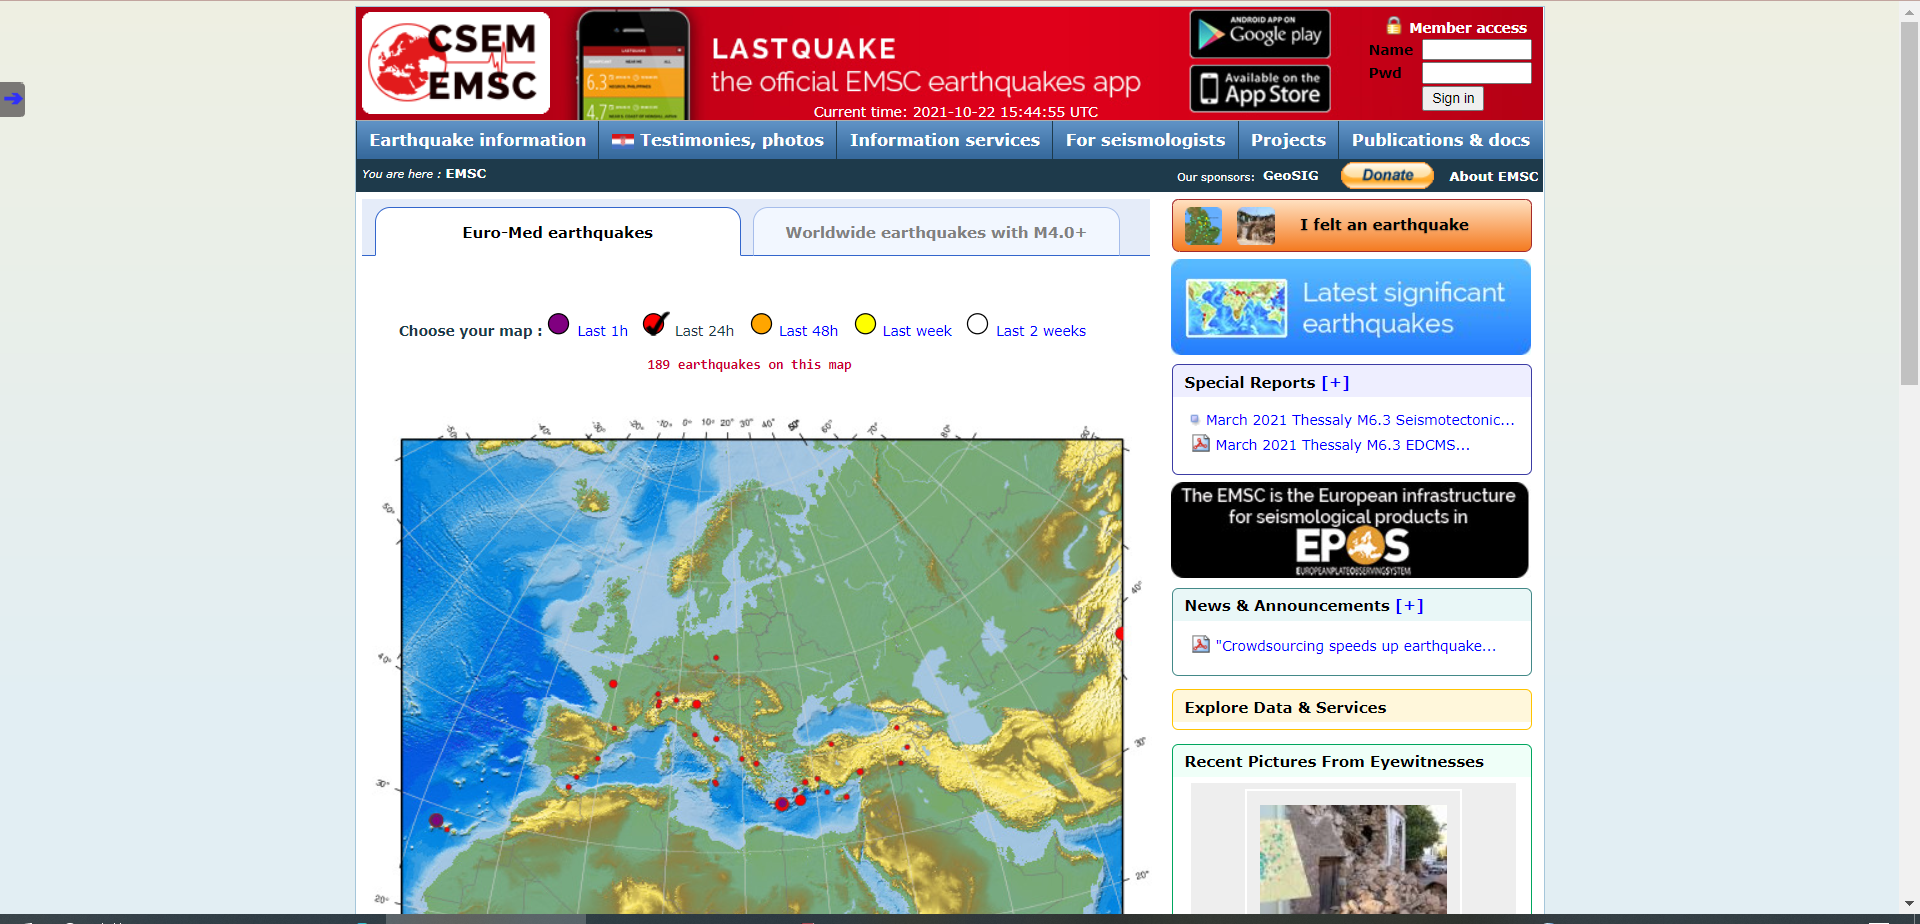
\includegraphics[width=\textwidth]{slike/emsc1.PNG} %veličina u odnosu na širinu linije
			\caption{Slika 2.2: početna stranica EMSC-a}
			\label{fig:promjene2} %label mora biti drugaciji za svaku sliku
		\end{figure}

{Prednost aplikacije „TectonicHR“ bila bi preglednost i mogućnost lakšeg snalaženja na karti. 
Mogućnost prijave seizmologa na stranicu omogućilo bi bolju prilagodbu stranice. Građanima pri korištenju ne bi smetali izbornici s mogućnostima koje oni ne bi koristili, već bi im se pregledno prikazivale funkcionalnosti dodavanja potresa i pregleda aktualnih i starijih potresa. }

{Interes za korištenjem aplikacije imat će i građani i znanstvena zajednica. Potresi uvelike utječu na psihičko stanje ljudi. 
Kada dođe do potresa, većina želi znati gdje je epicentar, koliko je magnitude potres bio, kakvu je štetu prouzročilo u ostalim dijelovima pogođenog područja… 
Tako da bi ova jednostavna aplikacija ljudima pružila, za početak, osnovne informacije o doživljenom potresu te odgovor na neka od pitanja koja im se nameću nakon doživljenog potresa. 
Osim toga, korist od aplikacije imaju i znanstvenici koji putem opažanja građana mogu doći do vrlo vrijednih informacija. }\\		
		
\eject
		
	
	\chapter{Specifikacija programske potpore}
		
	\section{Funkcionalni zahtjevi}
			
			\textbf{\textit{dio 1. revizije}}\\
			
			\textit{Navesti \textbf{dionike} koji imaju \textbf{interes u ovom sustavu} ili  \textbf{su nositelji odgovornosti}. To su prije svega korisnici, ali i administratori sustava, naručitelji, razvojni tim.}\\
				
			\textit{Navesti \textbf{aktore} koji izravno \textbf{koriste} ili \textbf{komuniciraju sa sustavom}. Oni mogu imati inicijatorsku ulogu, tj. započinju određene procese u sustavu ili samo sudioničku ulogu, tj. obavljaju određeni posao. Za svakog aktora navesti funkcionalne zahtjeve koji se na njega odnose.}\\
			
			
			\noindent \textbf{Dionici:}
			
			\begin{packed_enum}
				
				\item Dionik 1
				\item Dionik 2				
				\item ...
				
			\end{packed_enum}
			
			\noindent \textbf{Aktori i njihovi funkcionalni zahtjevi:}
			
			
			\begin{packed_enum}
				\item  \underbar{Neregistrirani/neprijavljeni korisnik (inicijator) može:}
				
				\begin{packed_enum}
					
					\item ispuniti upitnik ako je osjetio novi potres
					\item pregledati sve arhivirane potrese s:
					\begin{packed_enum}
						\item interaktivnom kartom Hrvatske 
						\item dodatnim informacijama (broj ispunjenih upitnika, datum, vrijeme, geografski položaj, dubina fokusa, magnituda i naziv područja)
					\end{packed_enum}
					\item pristupiti aktualnim potresima i:
					\begin{packed_enum}
						\item ispuniti upitnik
						\item pregledati već analizirane podatke (karta, broj ispunjenih upitnika, datum, vrijeme, itd.)
					\end{packed_enum}
					
				\end{packed_enum}
			
				\item  \underbar{Aktor 2 (sudionik) može:}
				
				\begin{packed_enum}
					
					\item funkcionalnost 1
					\item funkcionalnost 2
					
				\end{packed_enum}
			\end{packed_enum}
			
			\eject 
			
			
				
			\subsection{Obrasci uporabe}
				
				\textbf{\textit{dio 1. revizije}}
				
				\subsubsection{Opis obrazaca uporabe}
					\textit{Funkcionalne zahtjeve razraditi u obliku obrazaca uporabe. Svaki obrazac je potrebno razraditi prema donjem predlošku. Ukoliko u nekom koraku može doći do odstupanja, potrebno je to odstupanje opisati i po mogućnosti ponuditi rješenje kojim bi se tijek obrasca vratio na osnovni tijek.}\\
					

					\noindent \underbar{\textbf{UC$<$broj obrasca$>$ -$<$ime obrasca$>$}}
					\begin{packed_item}
	
						\item \textbf{Glavni sudionik: }$<$sudionik$>$
						\item  \textbf{Cilj:} $<$cilj$>$
						\item  \textbf{Sudionici:} $<$sudionici$>$
						\item  \textbf{Preduvjet:} $<$preduvjet$>$
						\item  \textbf{Opis osnovnog tijeka:}
						
						\item[] \begin{packed_enum}
	
							\item $<$opis korak jedan$>$
							\item $<$opis korak dva$>$
							\item $<$opis korak tri$>$
							\item $<$opis korak četiri$>$
							\item $<$opis korak pet$>$
						\end{packed_enum}
						
						\item  \textbf{Opis mogućih odstupanja:}
						
						\item[] \begin{packed_item}
	
							\item[2.a] $<$opis mogućeg scenarija odstupanja u koraku 2$>$
							\item[] \begin{packed_enum}
								
								\item $<$opis rješenja mogućeg scenarija korak 1$>$
								\item $<$opis rješenja mogućeg scenarija korak 2$>$
								
							\end{packed_enum}
							\item[2.b] $<$opis mogućeg scenarija odstupanja u koraku 2$>$
							\item[3.a] $<$opis mogućeg scenarija odstupanja  u koraku 3$>$
							
						\end{packed_item}
					\end{packed_item}
				
					
				\subsubsection{Dijagrami obrazaca uporabe}
					
					\textit{Prikazati odnos aktora i obrazaca uporabe odgovarajućim UML dijagramom. Nije nužno nacrtati sve na jednom dijagramu. Modelirati po razinama apstrakcije i skupovima srodnih funkcionalnosti.}
				\eject		
				
			\subsection{Sekvencijski dijagrami}
				
				\textbf{\textit{dio 1. revizije}}\\
				
				\textit{Nacrtati sekvencijske dijagrame koji modeliraju najvažnije dijelove sustava (max. 4 dijagrama). Ukoliko postoji nedoumica oko odabira, razjasniti s asistentom. Uz svaki dijagram napisati detaljni opis dijagrama.}
				\eject
	
		\section{Ostali zahtjevi}
		
			\textbf{\textit{dio 1. revizije}}\\
		 
			 \textit{Nefunkcionalni zahtjevi i zahtjevi domene primjene dopunjuju funkcionalne zahtjeve. Oni opisuju \textbf{kako se sustav treba ponašati} i koja \textbf{ograničenja} treba poštivati (performanse, korisničko iskustvo, pouzdanost, standardi kvalitete, sigurnost...). Primjeri takvih zahtjeva u Vašem projektu mogu biti: podržani jezici korisničkog sučelja, vrijeme odziva, najveći mogući podržani broj korisnika, podržane web/mobilne platforme, razina zaštite (protokoli komunikacije, kriptiranje...)... Svaki takav zahtjev potrebno je navesti u jednoj ili dvije rečenice.}
			 
			 
			 
	
	\chapter{Arhitektura i dizajn sustava}
		Arhitektura naše aplikacije, može se podijeliti na sljedeće komponente
	\begin{itemize}
		\item 	Server strana (\textit{backend})
		\item 	Klijent strana (\textit{frontend})
		\item 	Baza podataka (\textit{db})		
	\end{itemize}
	\textbf{Serverska strana} glavna je komponenta naše aplikacije. U njoj se nalazi programska logika koja se brine da se korisniku isporuči ono što je zatražio i da aplikacija radi u skladu sa zahtjevima. Komunikacija prema klijentskoj strani ostvarena je korištenjem GraphQL-a (za manipulaciju s API-jem), a komunikacija prema bazi podataka ORM-om (Object-Relational Mapping). Također smo koristili razred Prisma kojem se predaju parametri SQL upita. Prisma je biblioteka sa serverske strane koja pomaže pri čitanju i pisanju podataka u i iz baze podataka na siguran način (štiti od SQL injekcija).
	
	\textbf{Baza podataka} koju smo koristili je PostgreSQL. Kako bi izbjegli programske greške u SQLu te potencijalne ranjivosti (npr. SQL injekcija), za komunikaciju s bazom koristili smo \textit{TypeORM} kako bi programer izbjegao greške u SQL jeziku. \textit{TypeOrm} je podvrsta radnog okvira ORM prilagođen TypeScriptu i JavaScriptu. Kroz \textit{TypeORM} dobili smo i sustav za verzioniranje baze podataka "migracije" tako da možemo lakše i sigurnije raditi izmjene na bazi te dijeliti te izmjene između programera u timu i produkcijskih servera. 
	
	\textbf{Klijentska strana} je pruža grafičko sučelje za olakšan i intuitivan pristup uslugama aplikacije. Ovu komponentu možemo zamisliti kao posrednika u komunikaciji između korisnika i serverske strane aplikacije. U našem slučaju klijentska strana implementirana je kao SPA (Single Page Application) s \textit{React}-om. \textit{React} je JavaScript knjižnica koja olakšava oblikovanje korisničkog sučelja.\\
	
	\begin{figure}[H]
		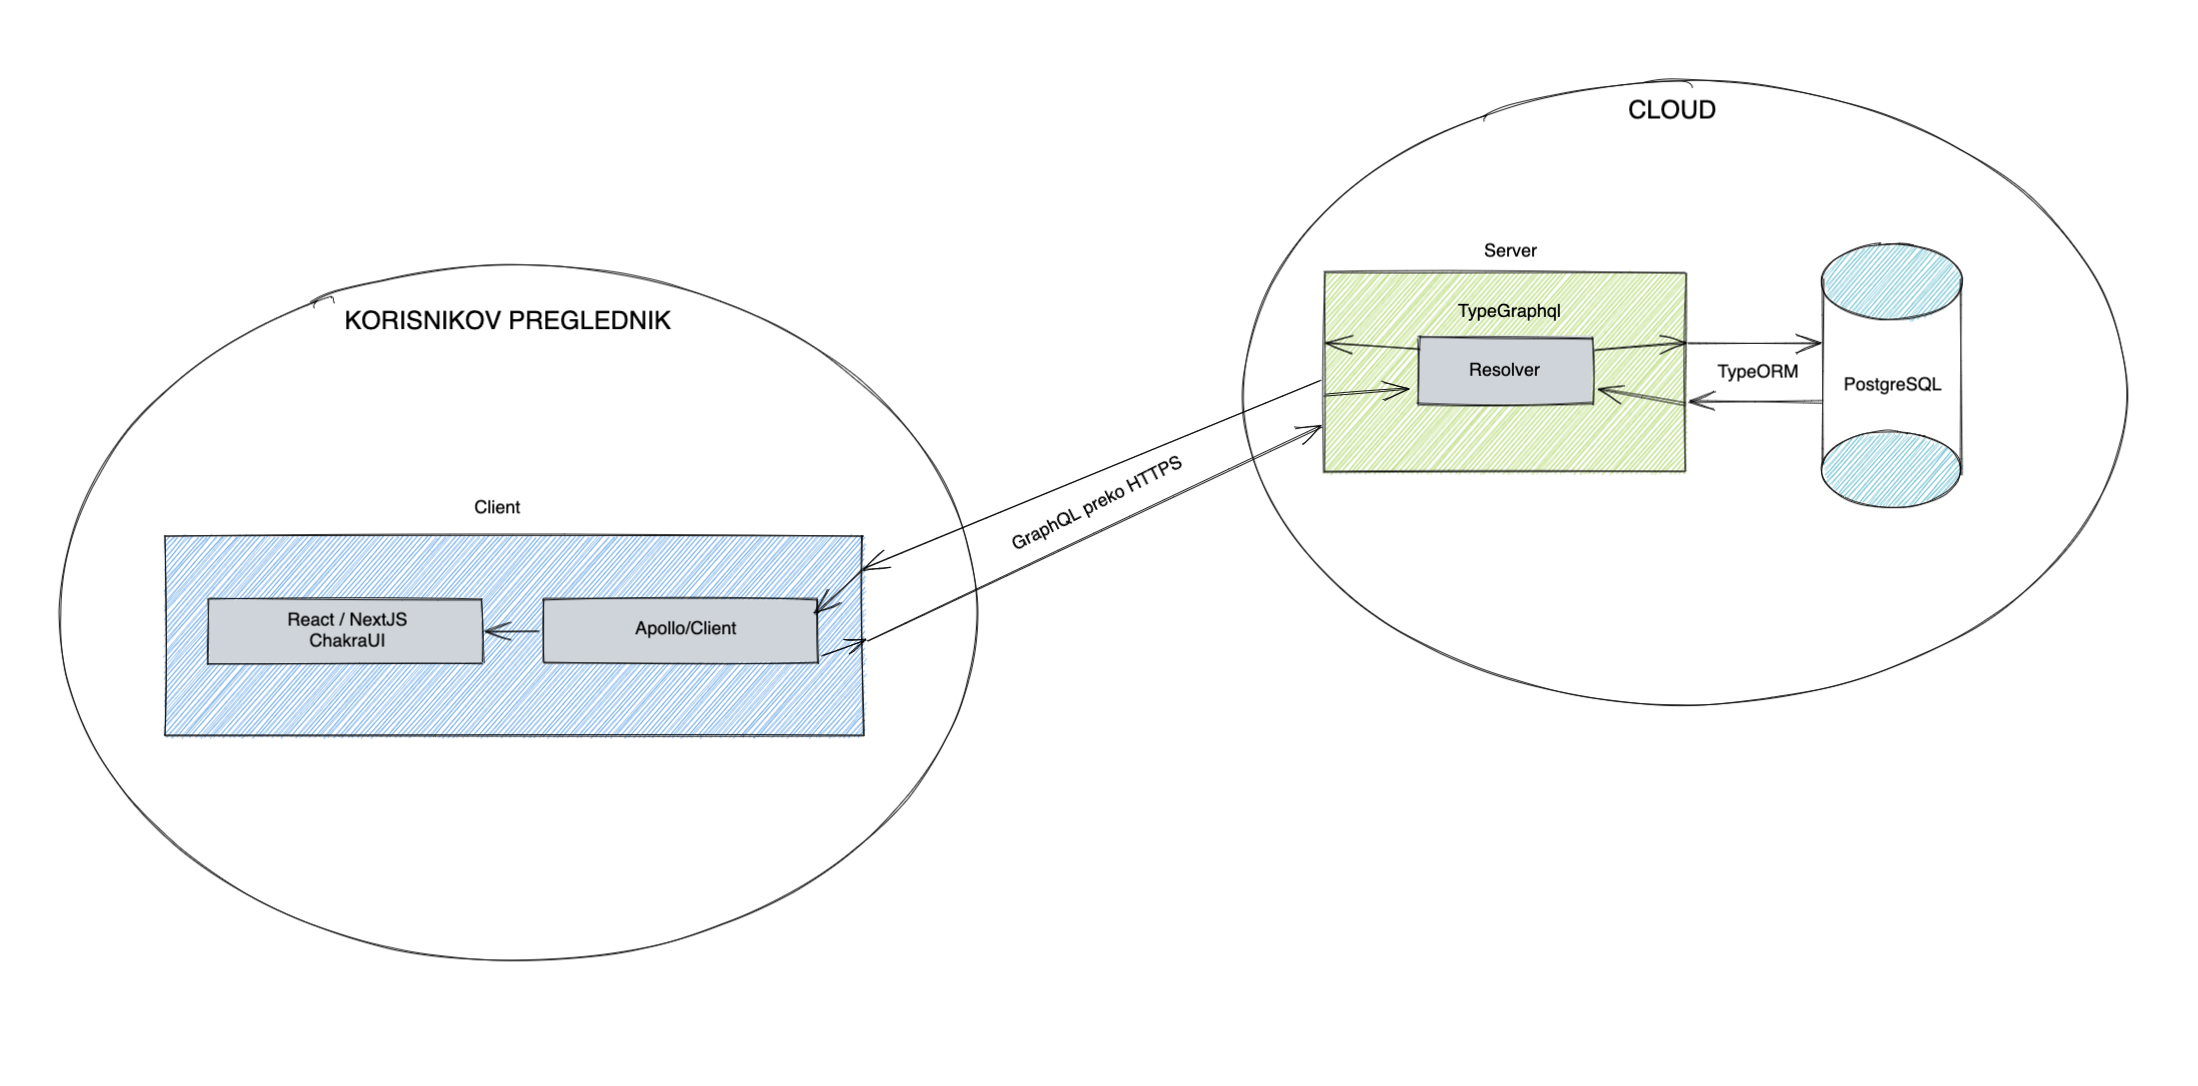
\includegraphics[width=\textwidth]{slike/arhitekturaDijagram.png} 
		\caption{Model arhitekture}
		\label{fig:arhitektura} 
	\end{figure}

				
		\section{Baza podataka}
		
		U našem sustavu korisimo PostgreSQL relacijsku bazu podataka za spremanje informacija o potresima i upitnicima. Zadaća baze podataka brza je i jednostavna pohrana, izmjena i dohvat podataka za daljnju obradu. Podaci će biti pohranjeni u tablice koje imaju svoje ime i atribute te će svaki entitet imati svoj primarni ključ, jedinstvenu
		oznakau svake n-torke koja ne smije imati vrijednost ”null”.
		U bazi podataka imamo sljedeće entitete:
		\begin{itemize}
			\item 	users
			\item 	earthquakes
			\item 	surveys
		\end{itemize}

			\subsection{Opis tablica}
			
				Tablica u kojoj se spremaju pristupni podaci te uloge korisnika u sustavu.
				\begin{longtblr}[
					label=none,
					entry=none
					]{
						width = \textwidth,
						colspec={|X[7,l]|X[7, l]|X[20, l]|}, 
						rowhead = 1,
					} %definicija širine tablice, širine stupaca, poravnanje i broja redaka naslova tablice
					\hline \multicolumn{3}{|c|}{\textbf{users}}	 \\ \hline[3pt]
					\SetCell{LightGreen}id & INT	&  	id korisnika  	\\ \hline
					created\_at	& TIMESTAMP &  vremenski žig kada je korisnik stvoren	\\ \hline 
					updated\_at	& TIMESTAMP &  vremenski žig kada je korisnik izmijenjen 	\\ \hline 
					email & VARCHAR &  email adresa korisnika \\ \hline 
					password\_hash & VARCHAR &  lozinka korisnika spremljena kao hash \\ \hline 
					role & Enum:UserRole &  uloga korisnika (admin i seizmolog) \\ \hline 
				\end{longtblr}

				Tablica u kojoj se spremaju prošli potresi, svaki potres može imati 0:n upitnika koje su građani ispunili.
				\begin{longtblr}[
					label=none,
					entry=none
					]{
						width = \textwidth,
						colspec={|X[7,l]|X[7, l]|X[20, l]|}, 
						rowhead = 1,
					} %definicija širine tablice, širine stupaca, poravnanje i broja redaka naslova tablice
					\hline \multicolumn{3}{|c|}{\textbf{earthquakes}}	 \\ \hline[3pt]
					\SetCell{LightGreen}id & INT	&  	id potresa  	\\ \hline
					created\_at	& TIMESTAMP &  vremenski žig kada je potres stvoren	\\ \hline 
					updated\_at	& TIMESTAMP &  vremenski žig kada je potres izmijenjen 	\\ \hline 
					name & VARCHAR &  naziv potresa \\ \hline 
					strength & REAL &  jačina potresa \\ \hline 
					epicenter\_lat & REAL &  geografska širina epicentra \\ \hline 
					epicenter\_lng & REAL &  geografska dužina epicentra \\ \hline 
					date	& TIMESTAMP &  vremenski žig kada se potres dogodio 	\\ \hline 
				\end{longtblr}

				Tablica u kojoj se nalaze ispunjeni upitnici.
				\begin{longtblr}[
					label=none,
					entry=none
					]{
						width = \textwidth,
						colspec={|X[7,l]|X[7, l]|X[20, l]|}, 
						rowhead = 1,
					} %definicija širine tablice, širine stupaca, poravnanje i broja redaka naslova tablice
					\hline \multicolumn{3}{|c|}{\textbf{surveys}}	 \\ \hline[3pt]
					\SetCell{LightGreen}id & INT	&  	id upitnika  	\\ \hline
					created\_at	& TIMESTAMP &  vremenski žig kada je upitnik stvoren	\\ \hline 
					updated\_at	& TIMESTAMP &  vremenski žig kada je upitnik izmijenjen 	\\ \hline 
					lat & REAL &  geografska širina upitnika \\ \hline 
					lng & REAL &  geografska dužina upitnika \\ \hline 
					\SetCell{LightBlue}earthquakeId	& INT &  id potresa za koji je ovaj upitnik ispunjen 	\\ \hline 
				\end{longtblr}

			
			\subsection{Dijagram baze podataka}

				\begin{figure}[H]
					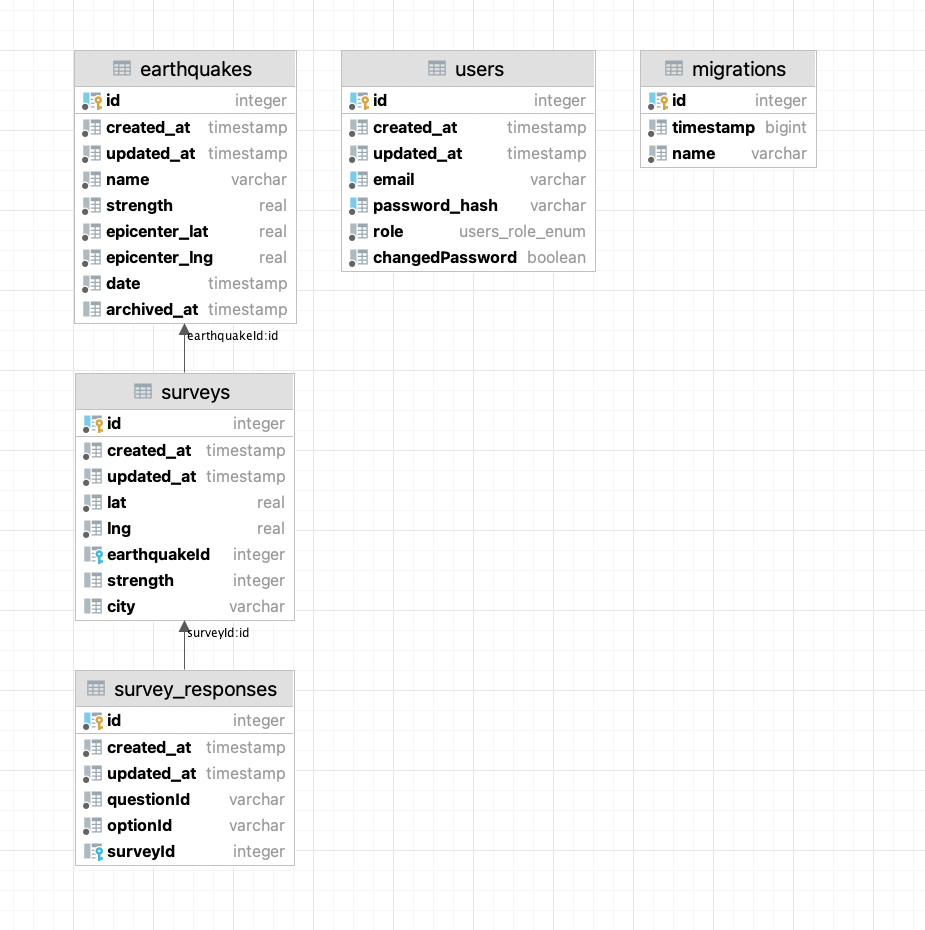
\includegraphics[width=\textwidth]{slike/tectonicDBDiagram.png} 
					\caption{Dijagram baze podataka}
					\label{fig:baza} 
				\end{figure}

			\eject
			
			
		\section{Dijagram razreda}
			
			\begin{figure}[H]
				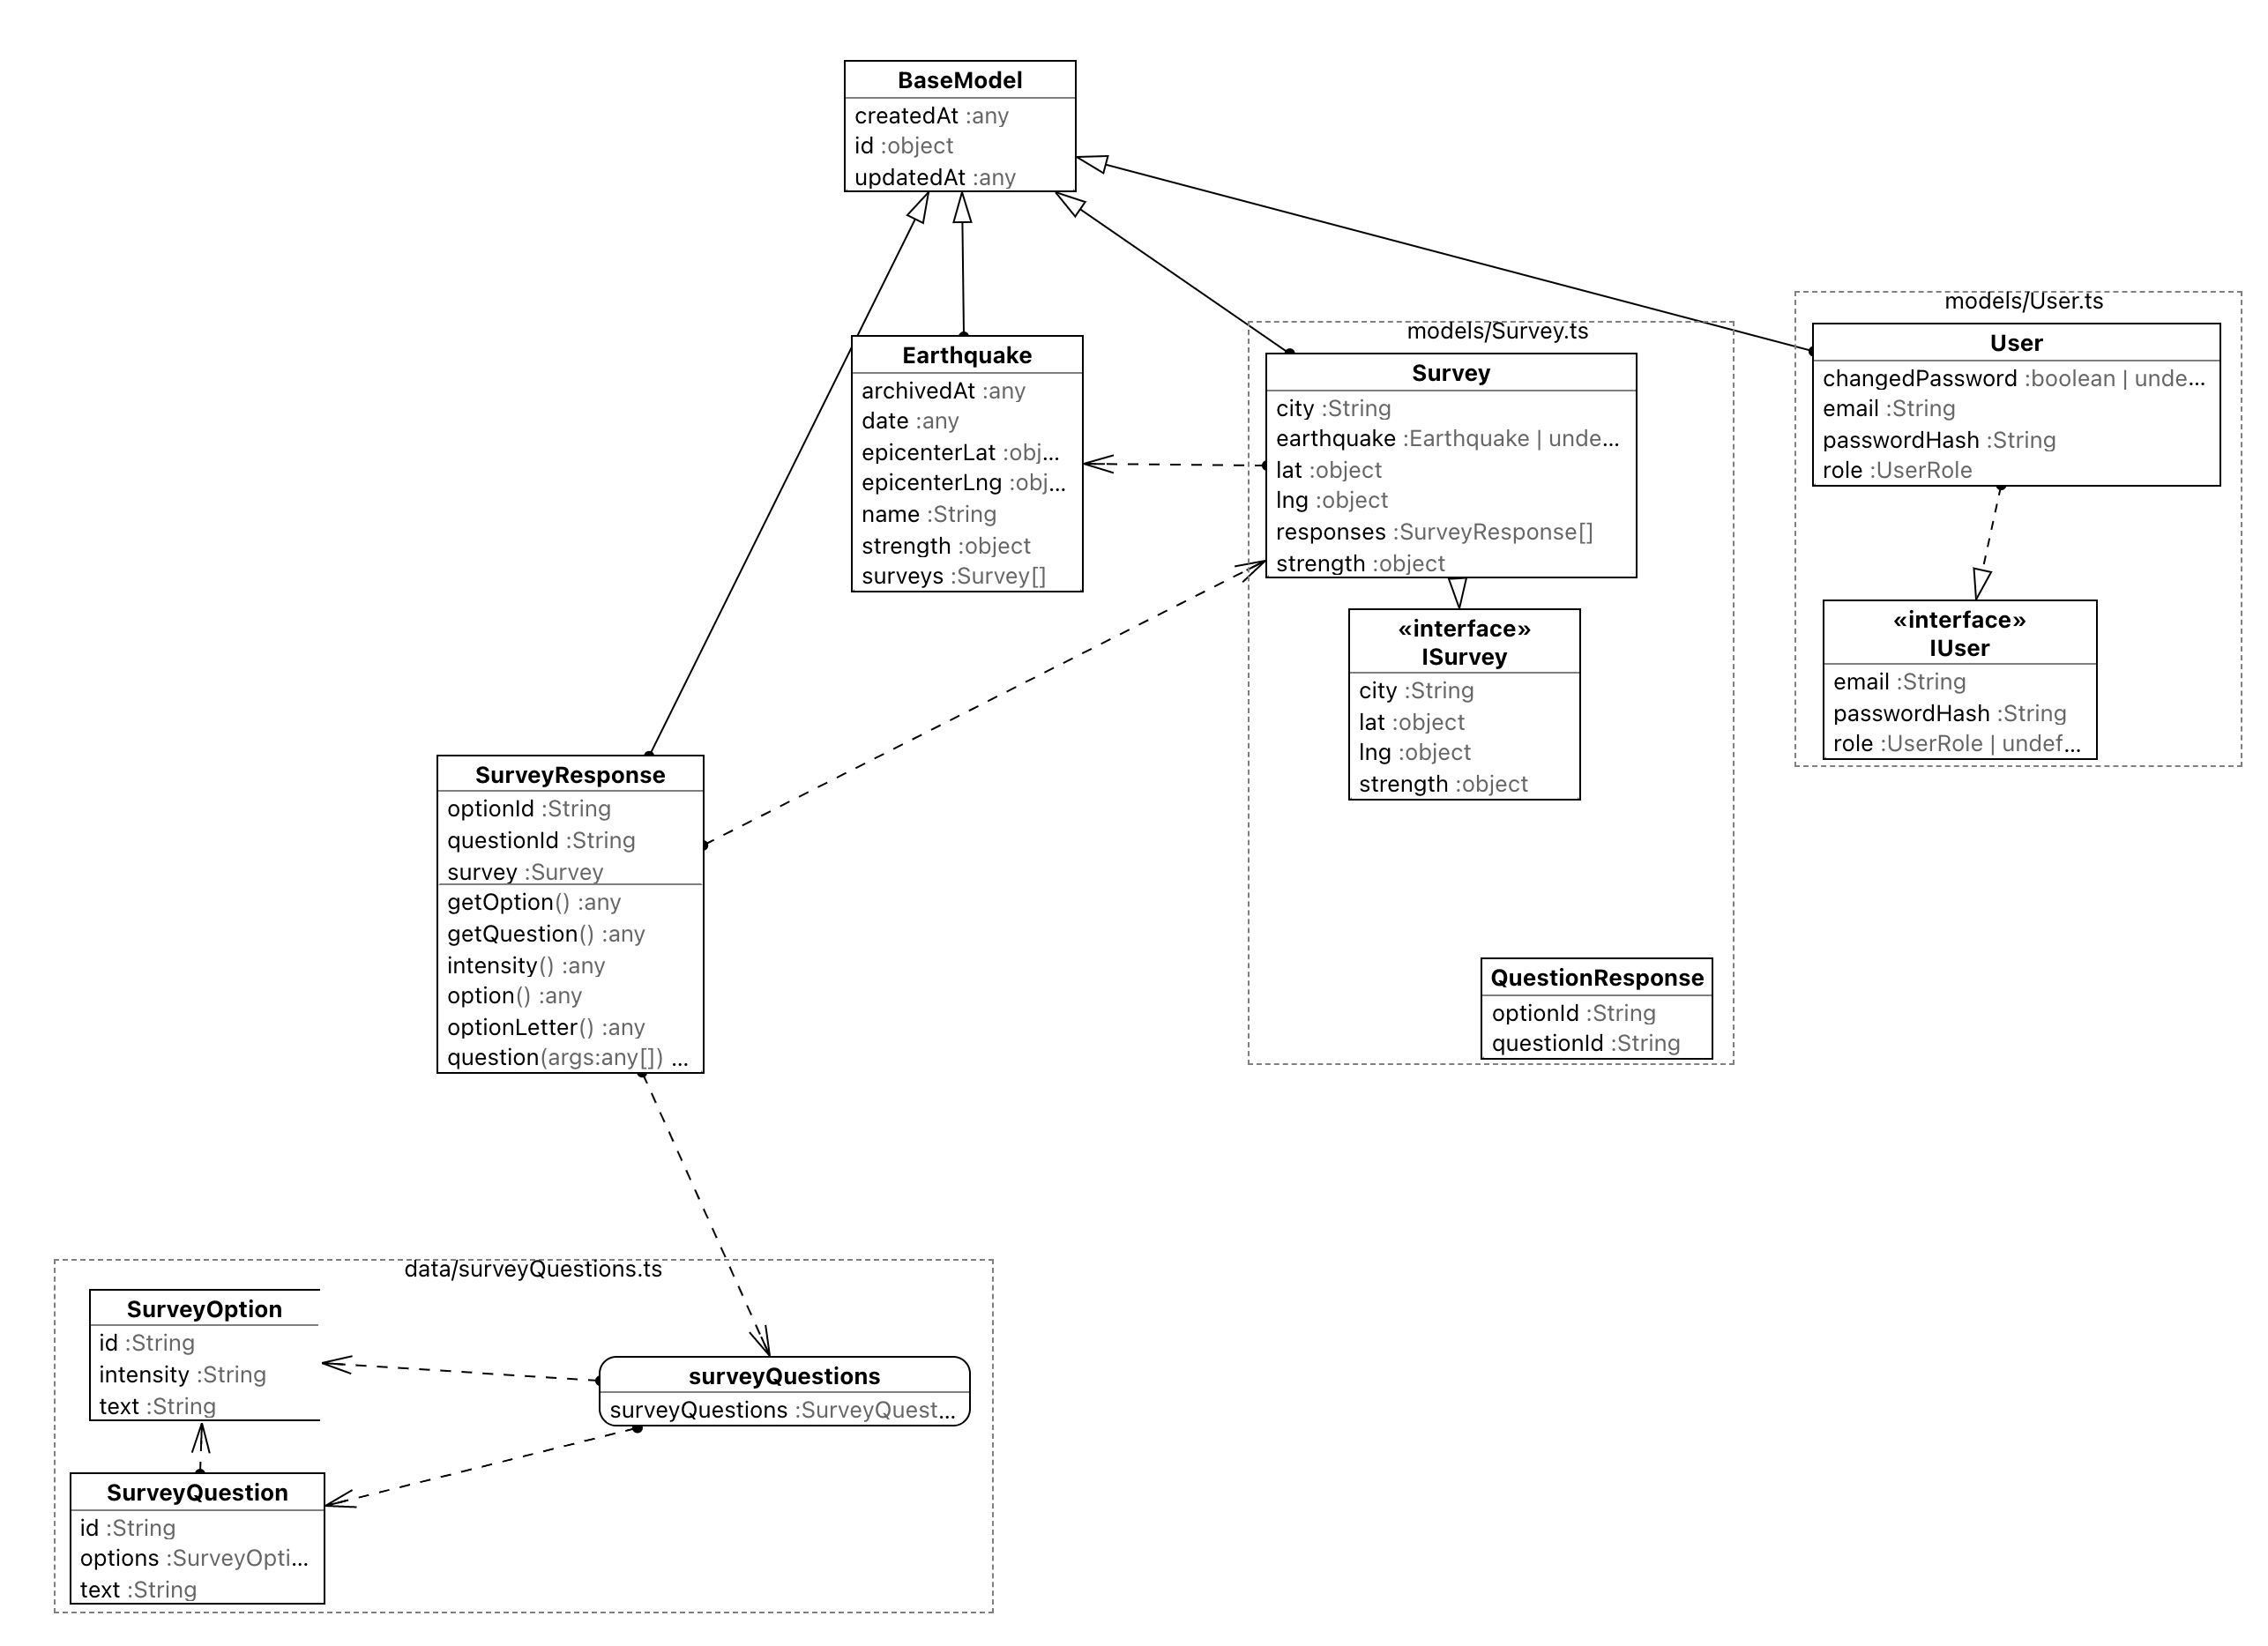
\includegraphics[width=\textwidth]{slike/classdiagram_only_db.png} 
				\caption{Dijagram razreda za modeliranje baze podataka}
				\label{fig:uml_db} 
			\end{figure}

			\begin{figure}[H]
				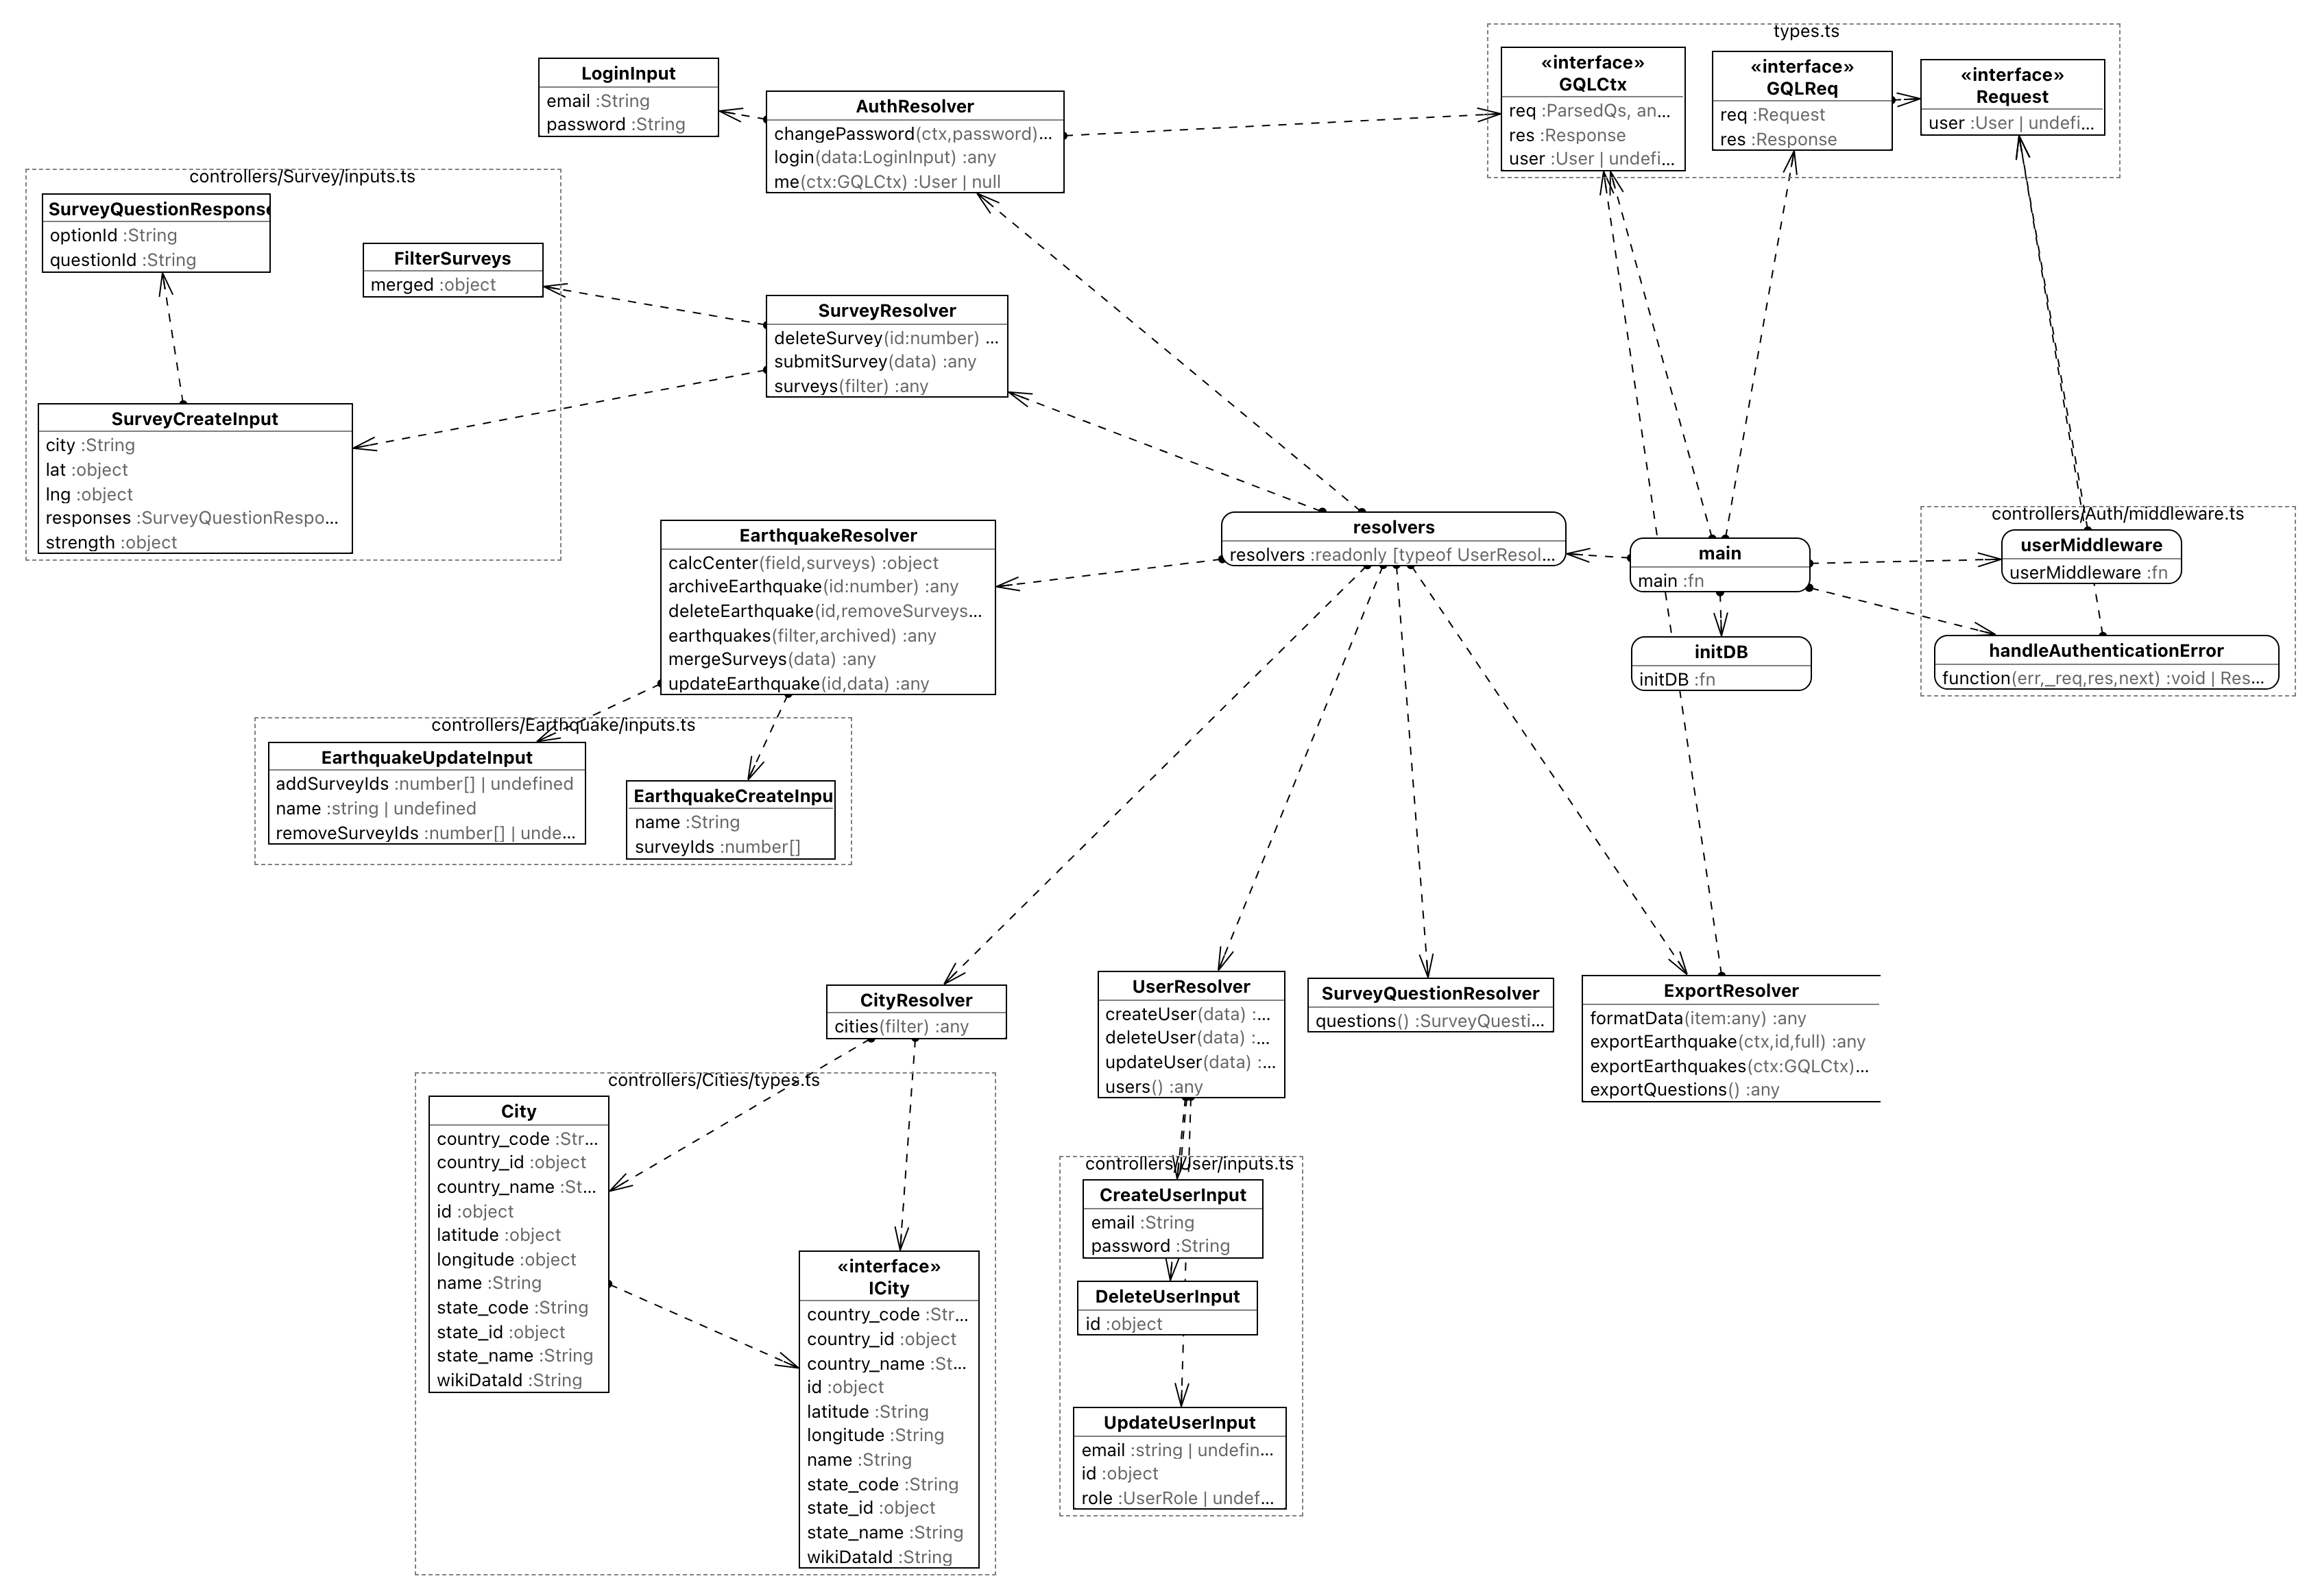
\includegraphics[width=\textwidth]{slike/classdiagram_no_db.png} 
				\caption{Dijagram razreda bez baze podataka}
				\label{fig:uml_no_db} 
			\end{figure}

			\begin{figure}[H]
				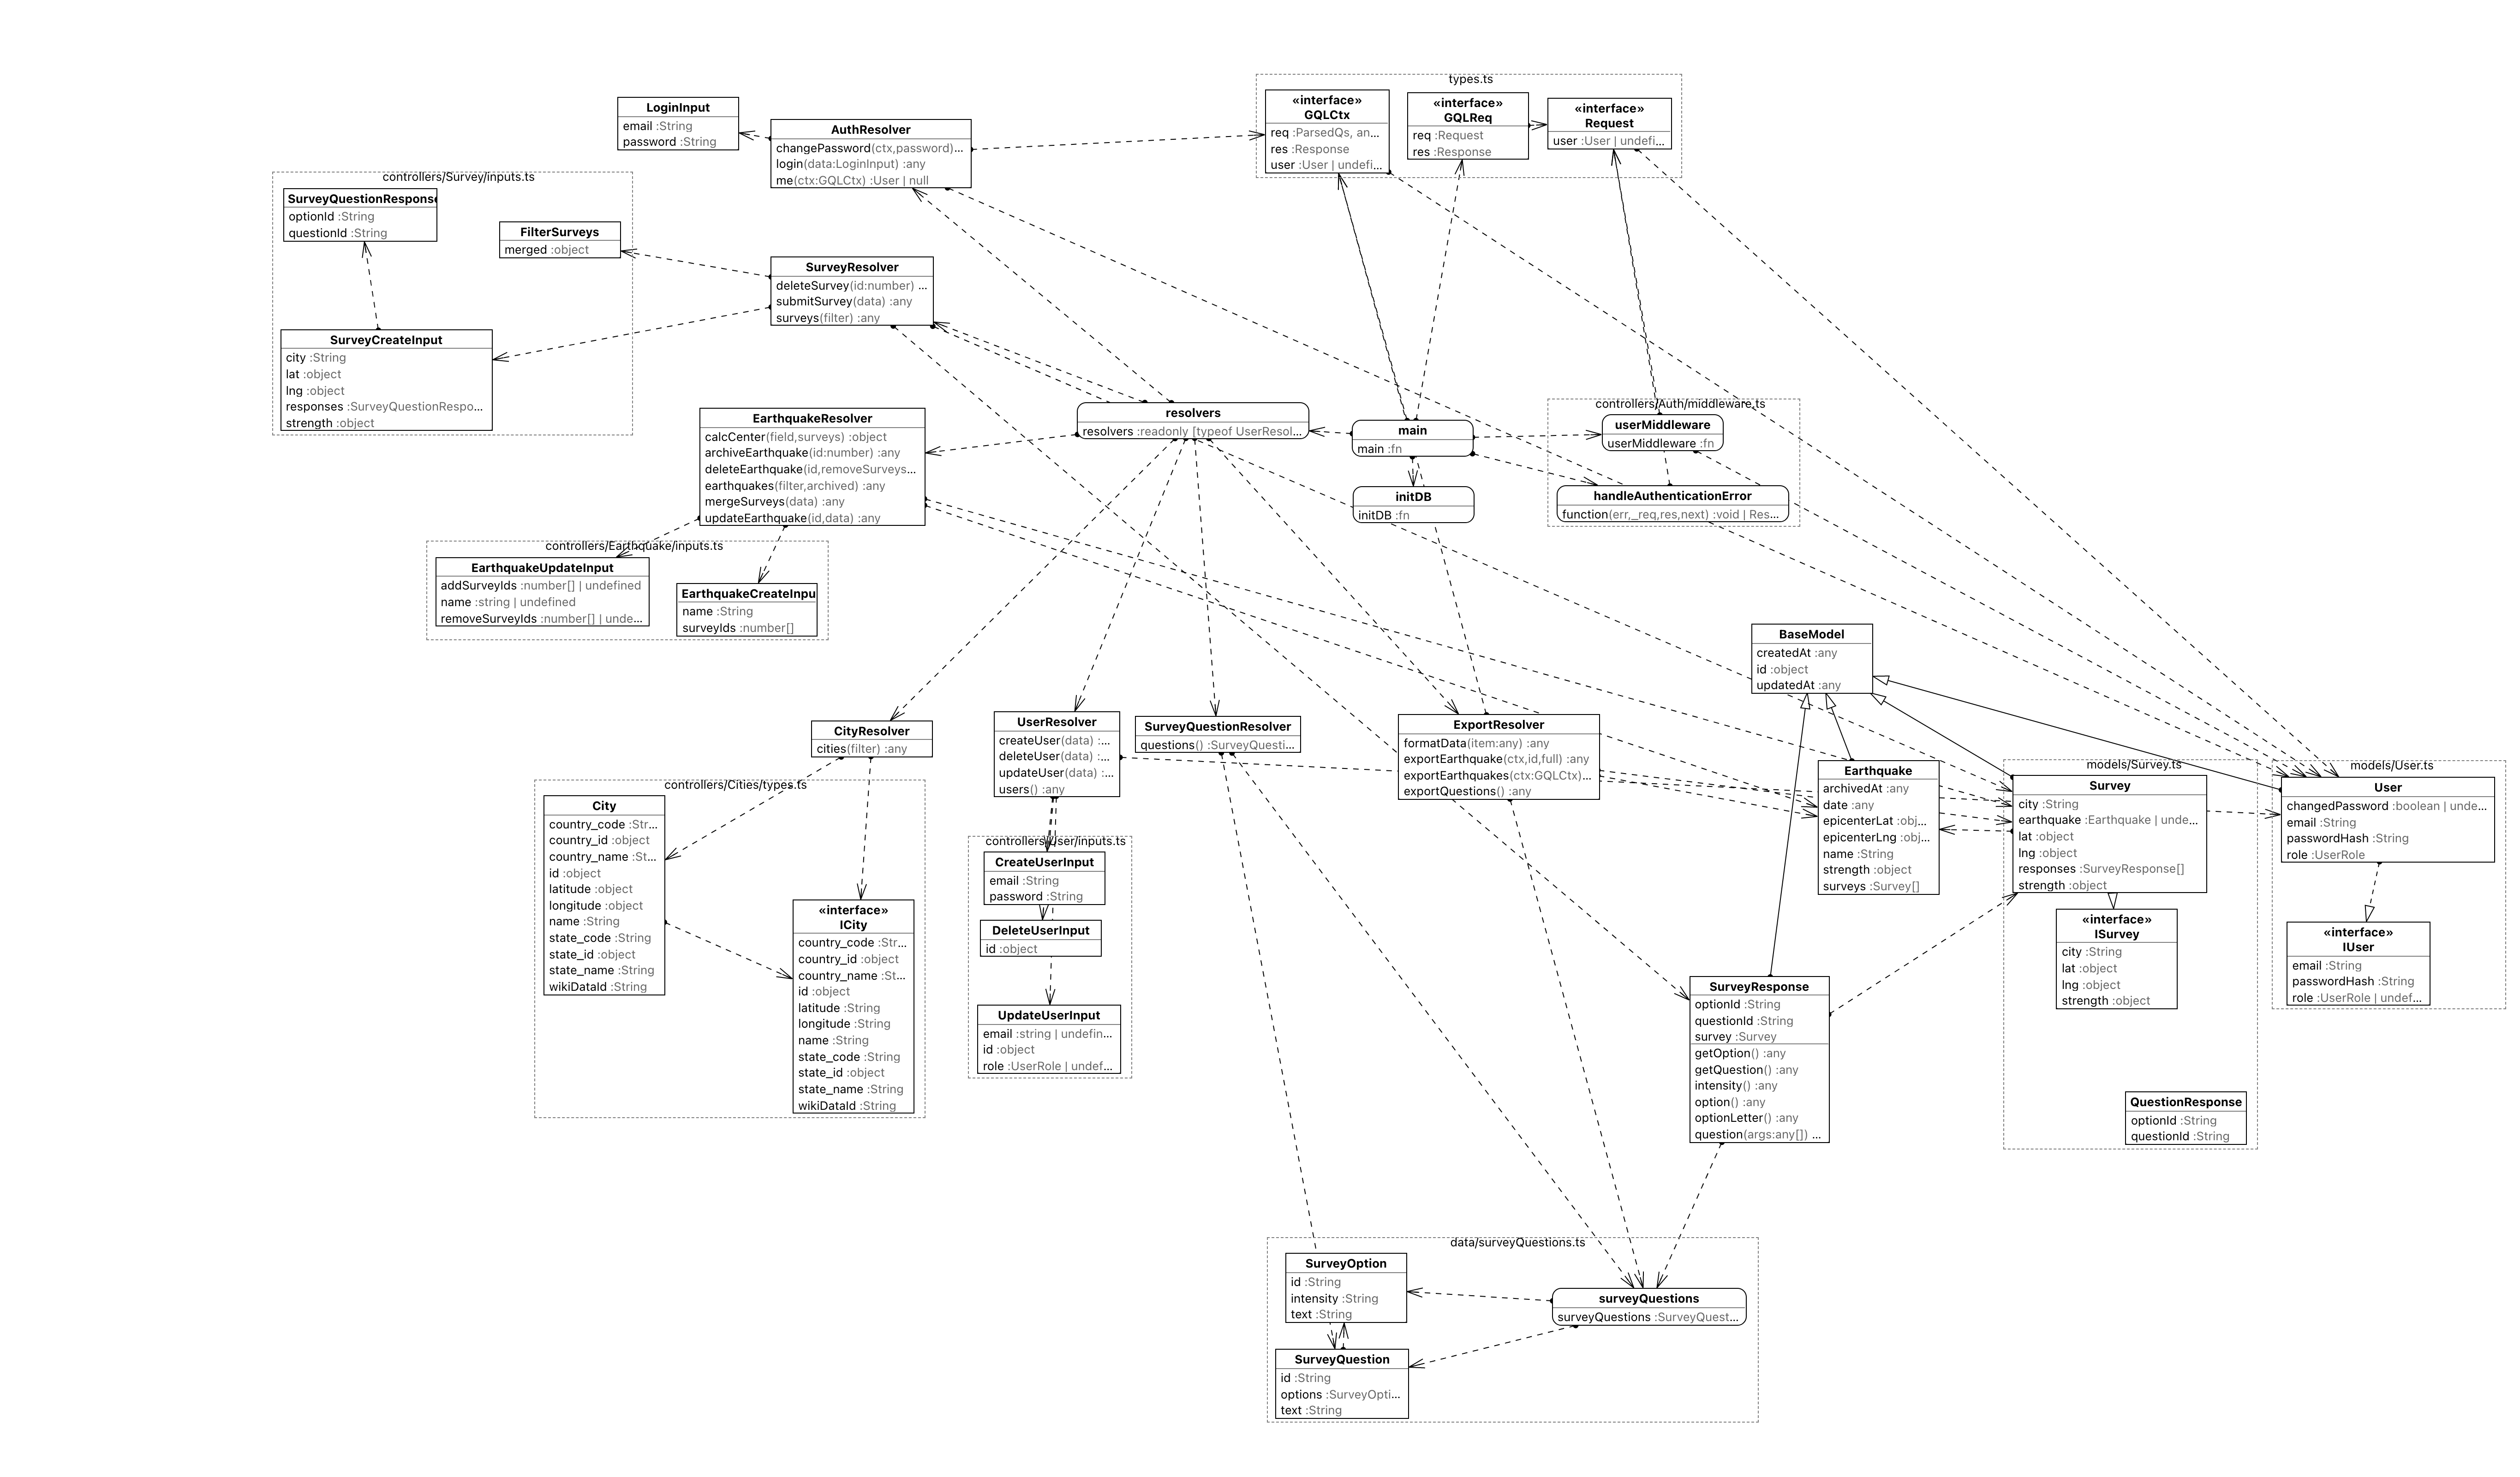
\includegraphics[width=\textwidth]{slike/classDiagram.png} 
				\caption{Dijagram razreda cijele aplikacije}
				\label{fig:uml} 
			\end{figure}

			\textbf{\textit{dio 2. revizije}}\\			
			
			\textit{Prilikom druge predaje projekta dijagram razreda i opisi moraju odgovarati stvarnom stanju implementacije}
			
			
			
			
			\eject
		
		\section{Dijagram stanja}
			
			
			\textbf{\textit{dio 2. revizije}}\\
			
			\textit{Potrebno je priložiti dijagram stanja i opisati ga. Dovoljan je jedan dijagram stanja koji prikazuje \textbf{značajan dio funkcionalnosti} sustava. Na primjer, stanja korisničkog sučelja i tijek korištenja neke ključne funkcionalnosti jesu značajan dio sustava, a registracija i prijava nisu. }
			
			
			\eject 
		
		\section{Dijagram aktivnosti}
			
			\textbf{\textit{dio 2. revizije}}\\
			
			 \textit{Potrebno je priložiti dijagram aktivnosti s pripadajućim opisom. Dijagram aktivnosti treba prikazivati značajan dio sustava.}
			
			\eject
		\section{Dijagram komponenti}
		
			\textbf{\textit{dio 2. revizije}}\\
		
			 \textit{Potrebno je priložiti dijagram komponenti s pripadajućim opisom. Dijagram komponenti treba prikazivati strukturu cijele aplikacije.}
		\eject
	\chapter{Implementacija i korisničko sučelje}
		
		
		\section{Korištene tehnologije i alati}
		Pisana komunikacija u timu odvijala se putem aplikacije WhatsApp\footnote{https://www.whatsapp.com/}, a sastanci putem Google Meeta\footnote{https://meet.google.com/} i Discorda\footnote{https://discord.com/}. WhatsApp je besplatna mobilna aplikacija koja služi za razmjenu poruka, fotografija i videozapisa putem mobilnog interneta pametnim telefonom. Google Meet je usluga videokomunikacije koju je razvio Google, dok je Discord VoIP aplikacija koja omogućava komunikaciju glasom, videom i tekstom.
		
		UML dijagrami napravljeni su alatom Visual Paradigm Online\footnote{https://online.visual-paradigm.com/}. Visual Paradigm Online je online alat za crtanje dijagrama i njihovu pohranu u web-pregledniku koji omogućava istovremeni rad više korisnika u stvarnom vremenu. Dijagrame možemo preuzeti u raznim formatima (.png, .jpeg, .pdf i dr.).
		
		Za vizualizaciju stranice korištena je Figma\footnote{https://www.figma.com/}, besplatan alat za UI i UX dizajn, uređivanje i izradu	prototipova te generiranje koda dostupan na webu ili u obliku desktop aplikacije.
		
		Izvornim kodom upravljano je sustavom Git\footnote{https://git-scm.com/}. Git je distribuirani sustav za upravljanje različitim	verzijama podataka (programskog koda, teksta i dr.). Sastoji se od udaljenog repozitorija koji se nalazi na nekoj Git platformi u oblaku i od lokalnih kopija tog repozitorija na računalima korisnika koji rade na projektu. Udaljeni repozitorij ovog projekta dostupan je na web platformi Gitlab\footnote{https://about.gitlab.com/}.
		
		Kao razvojno okruženje korišten je Visual Studio Code\footnote{https://code.visualstudio.com/}. Visual Studio Code
		je uređivač izvornog koda koji je razvio Microsoft za Linux, Windows i Mac OS platforme. Uključuje podršku za uklanjanje pogrešaka, isticanje sintakse, inteligentno dovršavanje koda, isječke, refaktoriranje koda i ugrađeni Git.
		
		Osim VSCode-a, koristili smo i JetBrains WebStorm\footnote{https://www.jetbrains.com/webstorm/} i JetBrains DataGrip\footnote{https://www.jetbrains.com/datagrip/}. WebStorm je integrirana razvojna okolina za JavaScript i povezane tehnologije, a DataGrip detektira moguće \textit{buggove} u kodu i predlaže najbolje opcije za njihovo ispravljanje.
		
		Cijeli sustav pisan je jezikom TypeScript\footnote{https://www.typescriptlang.org/} koji je proširenje jezika JavaScript(JavaScript s tipovima), skriptnog programskog jezika koji omogućava interakciju korisnika s web-stranicom.
		
		Za frontend smo koristili React\footnote{https://reactjs.org/} i Chakra UI\footnote{https://chakra-ui.com/}. React je knjižnica koja služi za izgradnju korisničkog sučelja ili UI komponenti, a Chakra je jednostavna modularna bibloteka komponenata	u kojoj se nalaze blokovi potrebni za izgradnju React aplikacija.
		
		 PostgreSQL\footnote{https://www.postgresql.org/} baza podataka spremljena je na $Heroku^{14}$	koji je ujedno i server. PostgreSQL je besplatni i relacijski sustav upravljanja bazom podataka otvorenog koda dizajniran za upravljanje nizom radnih opterećenja, od pojedinačnih strojeva do skladišta podataka ili web-usluga s mnogim istovremenim korisnicima. Heroku je platforma u oblaku, točnije platforma kao usluga (engl. Platform as a Service, skraćeno PaaS), što znači da korisnici	na nju postavljaju ili na njoj izraduju aplikaciju koja će se na njoj i izvršavati.
		
			\eject 
		
	
		\section{Ispitivanje programskog rješenja}
			
			\textbf{\textit{dio 2. revizije}}\\
			
			 \textit{U ovom poglavlju je potrebno opisati provedbu ispitivanja implementiranih funkcionalnosti na razini komponenti i na razini cijelog sustava s prikazom odabranih ispitnih slučajeva. Studenti trebaju ispitati temeljnu funkcionalnost i rubne uvjete.}
	
			
			\subsection{Ispitivanje komponenti}
			\textit{Potrebno je provesti ispitivanje jedinica (engl. unit testing) nad razredima koji implementiraju temeljne funkcionalnosti. Razraditi \textbf{minimalno 6 ispitnih slučajeva} u kojima će se ispitati redovni slučajevi, rubni uvjeti te izazivanje pogreške (engl. exception throwing). Poželjno je stvoriti i ispitni slučaj koji koristi funkcionalnosti koje nisu implementirane. Potrebno je priložiti izvorni kôd svih ispitnih slučajeva te prikaz rezultata izvođenja ispita u razvojnom okruženju (prolaz/pad ispita). }
			
			
			
			\subsection{Ispitivanje sustava}
			
			 \textit{Potrebno je provesti i opisati ispitivanje sustava koristeći radni okvir Selenium\footnote{\url{https://www.seleniumhq.org/}}. Razraditi \textbf{minimalno 4 ispitna slučaja} u kojima će se ispitati redovni slučajevi, rubni uvjeti te poziv funkcionalnosti koja nije implementirana/izaziva pogrešku kako bi se vidjelo na koji način sustav reagira kada nešto nije u potpunosti ostvareno. Ispitni slučaj se treba sastojati od ulaza (npr. korisničko ime i lozinka), očekivanog izlaza ili rezultata, koraka ispitivanja i dobivenog izlaza ili rezultata.\\ }
			 
			 \textit{Izradu ispitnih slučajeva pomoću radnog okvira Selenium moguće je provesti pomoću jednog od sljedeća dva alata:}
			 \begin{itemize}
			 	\item \textit{dodatak za preglednik \textbf{Selenium IDE} - snimanje korisnikovih akcija radi automatskog ponavljanja ispita	}
			 	\item \textit{\textbf{Selenium WebDriver} - podrška za pisanje ispita u jezicima Java, C\#, PHP koristeći posebno programsko sučelje.}
			 \end{itemize}
		 	\textit{Detalji o korištenju alata Selenium bit će prikazani na posebnom predavanju tijekom semestra.}
			
			\eject 
		
		
		\section{Dijagram razmještaja}
			
			\textbf{\textit{dio 2. revizije}}
			
			 \textit{Potrebno je umetnuti \textbf{specifikacijski} dijagram razmještaja i opisati ga. Moguće je umjesto specifikacijskog dijagrama razmještaja umetnuti dijagram razmještaja instanci, pod uvjetom da taj dijagram bolje opisuje neki važniji dio sustava.}
			
			\eject 
		
		\section{Upute za puštanje u pogon}
		
			\textbf{\textit{dio 2. revizije}}\\
		
			 \textit{U ovom poglavlju potrebno je dati upute za puštanje u pogon (engl. deployment) ostvarene aplikacije. Na primjer, za web aplikacije, opisati postupak kojim se od izvornog kôda dolazi do potpuno postavljene baze podataka i poslužitelja koji odgovara na upite korisnika. Za mobilnu aplikaciju, postupak kojim se aplikacija izgradi, te postavi na neku od trgovina. Za stolnu (engl. desktop) aplikaciju, postupak kojim se aplikacija instalira na računalo. Ukoliko mobilne i stolne aplikacije komuniciraju s poslužiteljem i/ili bazom podataka, opisati i postupak njihovog postavljanja. Pri izradi uputa preporučuje se \textbf{naglasiti korake instalacije uporabom natuknica} te koristiti što je više moguće \textbf{slike ekrana} (engl. screenshots) kako bi upute bile jasne i jednostavne za slijediti.}
			
			
			 \textit{Dovršenu aplikaciju potrebno je pokrenuti na javno dostupnom poslužitelju. Studentima se preporuča korištenje neke od sljedećih besplatnih usluga: \href{https://aws.amazon.com/}{Amazon AWS}, \href{https://azure.microsoft.com/en-us/}{Microsoft Azure} ili \href{https://www.heroku.com/}{Heroku}. Mobilne aplikacije trebaju biti objavljene na F-Droid, Google Play ili Amazon App trgovini.}
			
			
			\eject 
	\chapter{Zaključak i budući rad}
		
				Naš tim radio je na razvoju web aplikacije TectonicHR koja služi olakšanom prikupljanju i prikazu podataka o potresima. Korisnike koji pristupaju aplikaciji podijelili smo u tri kategorije: administrator, građani (neregistrirani korisnici) i seizmolozi (korisnici koje registrira administrator). Potrese smo podijelili na arhivirane i aktualne. Aktualni potresi su oni za koje se još mogu ispuniti upitnici. Kada administrator arhivira neki potres, on prelazi u arhivirane potrese te se za njega više ne može ispuniti upitnik. Korisnici mogu ispuniti upitnik i za neki potres koji još nije ni u arhiviranim ni u aktualnim potresima. Na taj način oni prijavljuju novi potres. Na temelju odgovora iz upitnika računa se intenzitet potresa te se potresi prikazuju na karti bojom koja ovisi o njihovom intenzitetu.
		
		Prije početka razvoja aplikacije, tim se morao sastati i razjasniti temu zadatka nakon čega je slijedila okvirna podjela poslova (tko bi htio raditi koji dio). Pri dio rada tima više se fokusirao na dokumentaciju projekta. Upravo ta detaljna analiza zahtjeva aplikacije kasnije je olakšala izradu same aplikacije. Ova faza rada uključivala je dokumentiranje funkcionalnih i nefunkcionalnih zahtjeva, razradu obrazaca uporabe te crtanje dijagrama (dijagram obrazaca uporabe, sekvencijski dijagram, dijagram razreda, model baze podataka). Za izradu dijagrama i dokumentiranje projekta bilo je potrebno znanje s predavanja predmeta te se svaki dio dokumentacije pisao nakon što bi bio ispričan na predavanju. U prvom dijelu rada na projektu također smo izradili prototip u Figmi koji nam je dao ideju izgleda konačne verzije aplikacije i olakšao u izradi frontenda.
		
		Druga faza projekta više se orijentirala na pisanje koda. Za izradu frontenda se koristio React što je većini članova bilo nepoznato te je zahtijevalo više samostalnog i ubrzanog
		učenja. Obrasci i dijagrami izrađeni u prvoj fazi su uvelike pomogli u izradi frontenda i backenda jer su
		pokazali kako bi se aplikacija trebala komunicirati s korisnikom te odrediti gdje smije pristupiti, a gdje ne jer nemaju svi korisnici ista prava i mogućnosti u aplikaciji. U ovoj fazi smo dokumentirali dijagram stanja, dijagram aktivnosti i dijagram komponenti. 
		
		 \textit{Potrebno je točno popisati funkcionalnosti koje nisu implementirane u ostvarenoj aplikaciji.}
		
		\eject 
	\chapter*{Popis literature}
		\addcontentsline{toc}{chapter}{Popis literature}
	 	
 		\textbf{\textit{Kontinuirano osvježavanje}}
	
		\textit{Popisati sve reference i literaturu koja je pomogla pri ostvarivanju projekta.}
		
		
		\begin{enumerate}
			
			
			\item  Programsko inženjerstvo, FER ZEMRIS, \url{http://www.fer.hr/predmet/proinz}
			
			\item  I. Sommerville, "Software engineering", 8th ed, Addison Wesley, 2007.
			
			\item  T.C.Lethbridge, R.Langaniere, "Object-Oriented Software Engineering", 2nd ed. McGraw-Hill, 2005.
			
			\item  I. Marsic, Software engineering book``, Department of Electrical and Computer Engineering, Rutgers University, \url{http://www.ece.rutgers.edu/~marsic/books/SE}
			
			\item  The Unified Modeling Language, \url{https://www.uml-diagrams.org/}
			
			\item  Astah Community, \url{http://astah.net/editions/uml-new}
			
			\item EMSC, \url{https://www.emsc-csem.org/#2}
			
			\item TypeGraphql dokumentacija, \url{https://typegraphql.com/}

            \item GraphQL dokumentacija, \url{https://graphql.org/}

            \item Apollo client dokumentacija, \url{https://www.apollographql.com/docs/react/}

            \item ChakraUI dokumentacija, \url{https://chakra-ui.com/}

            \item TypeORM dokumentacija, \url{https://typeorm.io/}

		\end{enumerate}
		
		 
	
	
	\begingroup
	\renewcommand*\listfigurename{Indeks slika i dijagrama}
	%\renewcommand*\listtablename{Indeks tablica}
	%\let\clearpage\relax
	\listoffigures
	%\vspace{10mm}
	%\listoftables
	\endgroup
	\addcontentsline{toc}{chapter}{Indeks slika i dijagrama}


	
	\eject 
		
	\chapter*{Dodatak: Prikaz aktivnosti grupe}
		\addcontentsline{toc}{chapter}{Dodatak: Prikaz aktivnosti grupe}
		
		\section*{Dnevnik sastajanja}
		
		\textbf{\textit{Kontinuirano osvježavanje}}\\
		
		 \textit{U ovom dijelu potrebno je redovito osvježavati dnevnik sastajanja prema predlošku.}
		
		\begin{packed_enum}
			\item  sastanak
			
			\item[] \begin{packed_item}
				\item Datum: 9.10.2021.
				\item Prisustvovali: M.Ćurković, D.Čemeljić, A.Engler, K.Iličić, D.Vorkapić
				\item Teme sastanka:
				\begin{packed_item}
					\item  upoznavanje članova tima
				\end{packed_item}
			\end{packed_item}
			
			\item  sastanak
			\item[] \begin{packed_item}
				\item Datum: 19.10.2021.
				\item Prisustvovali: M.Ćurković, D.Čemeljić, A.Engler, K.Iličić, M.Jurić, D.Vorkapić, F.Zekan
				\item Teme sastanka:
				\begin{packed_item}
					\item  upoznavanje s korištenim tehnologijama
					\item  razjašnjavanje zahtjeva
					\item  razrada specifikacije programske potpore
				\end{packed_item}
			\end{packed_item}
		
			\item  sastanak
			\item[] \begin{packed_item}
				\item Datum: 26.10.2021.
				\item Prisustvovali: M.Ćurković, D.Čemeljić, A.Engler, K.Iličić, M.Jurić, D.Vorkapić
				\item Teme sastanka:
				\begin{packed_item}
					\item  dogovor o izgledu stranice
					\item  sastavljanje prototipa u alatu Figma
					\item  podjela zadataka
				\end{packed_item}
			\end{packed_item}
			
			%
			
		\end{packed_enum}
		
		\eject
		\section*{Tablica aktivnosti}
		
			\textbf{\textit{Kontinuirano osvježavanje}}\\
			
			 \textit{Napomena: Doprinose u aktivnostima treba navesti u satima po članovima grupe po aktivnosti.}

			\begin{longtblr}[
					label=none,
				]{
					vlines,hlines,
					width = \textwidth,
					colspec={X[7, l]X[1, c]X[1, c]X[1, c]X[1, c]X[1, c]X[1, c]X[1, c]}, 
					vline{1} = {1}{text=\clap{}},
					hline{1} = {1}{text=\clap{}},
					rowhead = 1,
				} 
				\multicolumn{1}{c|}{} & \multicolumn{1}{c|}{\rotatebox{90}{\textbf{Maja Jurić }}} & \multicolumn{1}{c|}{\rotatebox{90}{\textbf{David Čemeljić }}} &	\multicolumn{1}{c|}{\rotatebox{90}{\textbf{Mihovil Ćurković }}} & \multicolumn{1}{c|}{\rotatebox{90}{\textbf{Antonija Engler }}} &	\multicolumn{1}{c|}{\rotatebox{90}{\textbf{Klara Iličić }}} & \multicolumn{1}{c|}{\rotatebox{90}{\textbf{Dalijo Vorkapić }}} &	\multicolumn{1}{c|}{\rotatebox{90}{\textbf{Fran Zekan }}} \\  
				Upravljanje projektom 		&  &  &  &  &  &  & \\ 
				Opis projektnog zadatka 	&  &  &  &  &  &  & \\ 
				
				Funkcionalni zahtjevi       &  &  &  &  &  &  &  \\ 
				Opis pojedinih obrazaca 	&  3  &  &  &  3  &  3  &  &  \\ 
				Dijagram obrazaca 			&  &  &  &  &  &  &  \\ 
				Sekvencijski dijagrami 		&  &  &  &  &  &  &  \\ 
				Opis ostalih zahtjeva 		&  &  &  &  &  &  &  \\ 

				Arhitektura i dizajn sustava	 &  &  &  &  &  &  &  \\ 
				Baza podataka				&  &  &  &  &  &  &   \\ 
				Dijagram razreda 			&  &  &  &  &  &  &   \\ 
				Dijagram stanja				&  &  &  &  &  &  &  \\ 
				Dijagram aktivnosti 		&  &  &  &  &  &  &  \\ 
				Dijagram komponenti			&  &  &  &  &  &  &  \\ 
				Korištene tehnologije i alati 		&  &  &  &  &  &  &  \\ 
				Ispitivanje programskog rješenja 	&  &  &  &  &  &  &  \\ 
				Dijagram razmještaja			&  &  &  &  &  &  &  \\ 
				Upute za puštanje u pogon 		&  &  &  &  &  &  &  \\  
				Dnevnik sastajanja 			&  &  &  &  &  &  &  \\ 
				Zaključak i budući rad 		&  &  &  &  &  &  &  \\  
				Popis literature 			&  &  &  &  &  &  &  \\  
				&  &  &  &  &  &  &  \\ \hline 
				\textit{Dodatne stavke kako ste podijelili izradu aplikacije} 			&  &  &  &  &  &  &  \\ 
				\textit{npr. izrada početne stranice} 				&  &  &  &  &  &  &  \\  
				\textit{izrada baze podataka} 		 			&  &  &  &  &  &  & \\  
				\textit{spajanje s bazom podataka} 							&  &  &  &  &  &  &  \\ 
				\textit{back end} 							&  &  &  &  &  &  &  \\  
				 							&  &  &  &  &  &  &\\ 
			\end{longtblr}
					
					
		\eject
		\section*{Dijagrami pregleda promjena}
		
		\textbf{\textit{dio 2. revizije}}\\
		
		\textit{Prenijeti dijagram pregleda promjena nad datotekama projekta. Potrebno je na kraju projekta generirane grafove s gitlaba prenijeti u ovo poglavlje dokumentacije. Dijagrami za vlastiti projekt se mogu preuzeti s gitlab.com stranice, u izborniku Repository, pritiskom na stavku Contributors.}
		
	


\end{document} %naredbe i tekst nakon ove naredbe ne ulaze u izgrađen dokument 


